\chapter{Cài đặt và thực nghiệm}
\label{chap:thuc-nghiem}

Chương này trình bày việc cài đặt bốn phiên bản theo chiến lược ở Mục~\ref{sec:chien-luoc} và kết quả đo đạc. Thứ tự trình bày: môi trường đo, kiểm chứng tính đúng đắn, phiên bản OpenMP, hai kernel CUDA và cuối cùng là so sánh tổng hợp.

\section{Môi trường và phương pháp đo}
\label{sec:moi-truong}

Toàn bộ mã nguồn viết bằng C (bản CPU) và CUDA C++ (bản GPU), dùng chung các hàm khởi tạo, tính năng lượng và tham số dòng lệnh trong \code{src/nbody\_common.h}. Mã nguồn, số liệu thô và đồ thị nằm tại \url{https://github.com/doanh9a246-afk/motcongmotbangmay}. Bảng~\ref{tab:moi-truong} tóm tắt môi trường của phép đo tổng hợp.

\begin{table}[H]
\centering\small
\begin{tabular}{p{2.6cm}p{5.8cm}p{5.8cm}}
\toprule
 & \textbf{CPU} & \textbf{GPU} \\
\midrule
Phần cứng & Intel Core i5-12500H (4 lõi P + 8 lõi E, 16 luồng) & NVIDIA Tesla T4 (40 SM, Turing) trên Google Colab \\
Trình biên dịch & MinGW gcc 12.1, \code{-O3 -march=native -ffast-math -fopenmp} & nvcc 13.0, \code{-O3 -arch=sm\_75 -use\_fast\_math} \\
Cách đo & Mỗi cấu hình chạy 3 lần, lấy lần nhanh nhất; không tính khởi tạo, năng lượng, ghi file & Như CPU; có 1 lần warm-up kernel; thời gian H2D/D2H tính riêng \\
Tệp số liệu & \code{results/cpu\_laptop.csv} & \code{results/gpu\_t4.csv} \\
\bottomrule
\end{tabular}
\caption{Môi trường của phép đo tổng hợp CPU và GPU.}
\label{tab:moi-truong}
\end{table}

Ngoài phép đo tổng hợp, một số thí nghiệm riêng được đo trên máy của từng thành viên: thí nghiệm năng lượng trên Intel Core i5-12450HX (8 lõi/12 luồng, GCC 16.2), các thí nghiệm OpenMP chi tiết trên Intel Core i7-13620H (6 lõi P + 4 lõi E, 16 luồng, MinGW-W64 GCC 16.2). Cấu hình được ghi kèm từng thí nghiệm và trong các tệp \code{results/*.machine.txt}.

\section{Kiểm chứng tính đúng đắn}
\label{sec:dung-dan}

Mọi phiên bản dùng cùng trạng thái ban đầu (Plummer, seed 42) nên có thể so sánh trực tiếp kết quả. Chương trình có tùy chọn \code{-verify}: chạy bản cần kiểm tra và một bản tham chiếu từ cùng trạng thái đầu (bản CPU so với bản tuần tự, bản CUDA so với bản OpenMP), rồi so sánh vị trí của từng vật thể sau mô phỏng theo sai số tương đối lớn nhất (ngưỡng đạt: $10^{-4}$ cho CPU, $10^{-3}$ cho GPU). Bản OpenMP khớp bản tuần tự từng bit (sai số tương đối bằng 0) với 1, 2, 4 và 16 luồng; hai kernel CUDA khớp với sai số tương đối khoảng $10^{-8}$, đúng bậc sai số làm tròn của \code{float} khi dùng \code{rsqrtf}. Phép kiểm tra OpenMP và kiểm tra bảo toàn năng lượng ($|\Delta E/E_0|<10^{-3}$ sau 1000 bước) được chạy tự động mỗi khi có thay đổi mã nguồn.

\subsection{Thí nghiệm bảo toàn năng lượng}

Các phép đo dưới đây dùng $N=2048$, 2000 bước, seed 42, chế độ OpenMP với 12 luồng trên Intel Core i5-12450HX. Ở thí nghiệm \code{dt}, giữ $\varepsilon=0.01$; ở thí nghiệm \code{eps}, giữ $\Delta t=0.002$. Năng lượng được tính trước và sau mô phỏng bằng thế năng mềm $U_\varepsilon$ (Mục~\ref{sec:co-so-bai-toan}).

\begin{table}[H]
\centering\small
\begin{tabular}{lrrrr}
\toprule
\textbf{Thí nghiệm} & \textbf{Giá trị thay đổi} & \textbf{$\Delta t$} & \textbf{$\varepsilon$} & \textbf{$\lvert\Delta E/E_0\rvert$} \\
\midrule
\texttt{dt} & 0.0005 & 0.0005 & 0.01 & 1.700e-05 \\
\texttt{dt} & 0.001 & 0.001 & 0.01 & 1.750e-06 \\
\texttt{dt} & 0.002 & 0.002 & 0.01 & 2.685e-06 \\
\texttt{dt} & 0.005 & 0.005 & 0.01 & 9.308e-05 \\
\texttt{dt} & 0.01 & 0.01 & 0.01 & 1.260e-03 \\
\texttt{eps} & 0.001 & 0.002 & 0.001 & 4.799e-03 \\
\texttt{eps} & 0.0031623 & 0.002 & 0.0031623 & 1.228e-04 \\
\texttt{eps} & 0.01 & 0.002 & 0.01 & 2.685e-06 \\
\texttt{eps} & 0.0316228 & 0.002 & 0.0316228 & 1.816e-05 \\
\texttt{eps} & 0.1 & 0.002 & 0.1 & 6.772e-06 \\
\bottomrule
\end{tabular}
\caption{Độ lệch năng lượng theo bước thời gian và hệ số softening ($N=2048$, 2000 bước).}
\label{tab:nang-luong}
\end{table}

Đồ thị log--log tương ứng là Hình~\ref{fig:vvduong_energy_dt} và Hình~\ref{fig:vvduong_energy_eps}.

\begin{figure}[H]
\centering
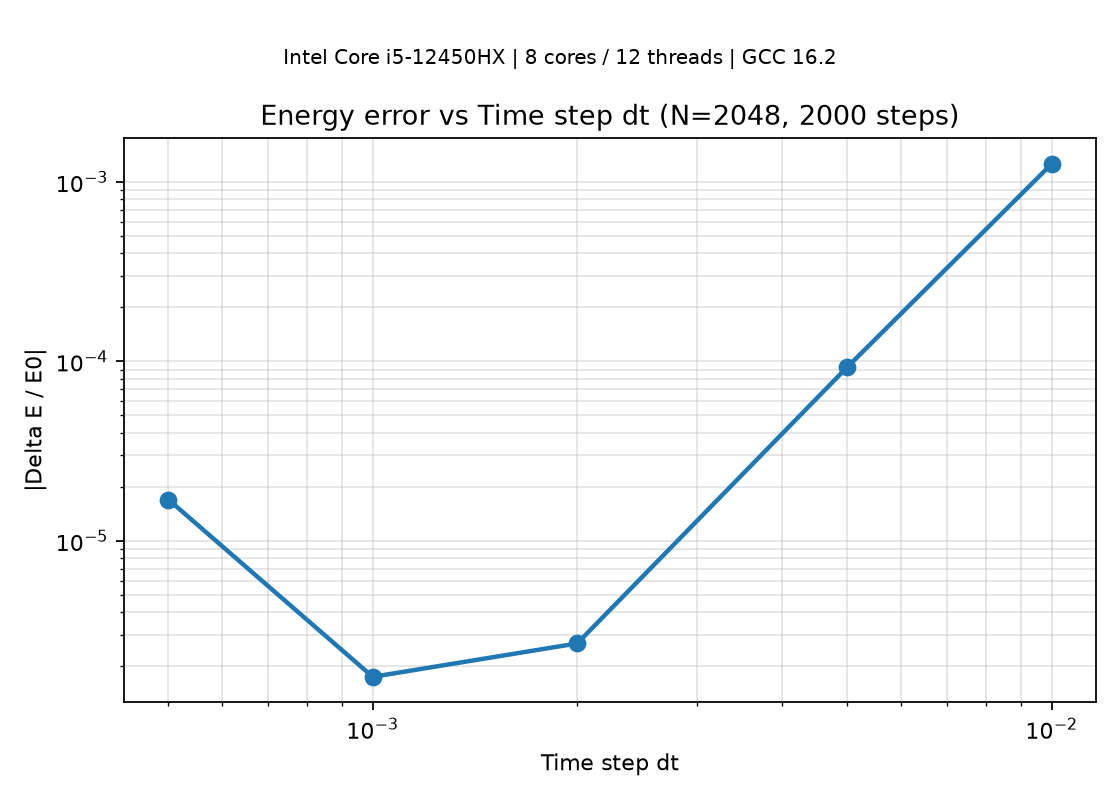
\includegraphics[width=0.85\linewidth]{vvduong_energy_dt}
\caption{Độ lệch năng lượng $|\Delta E/E_0|$ theo $\Delta t$ ($\varepsilon=0.01$).}
\label{fig:vvduong_energy_dt}
\end{figure}

\begin{figure}[H]
\centering
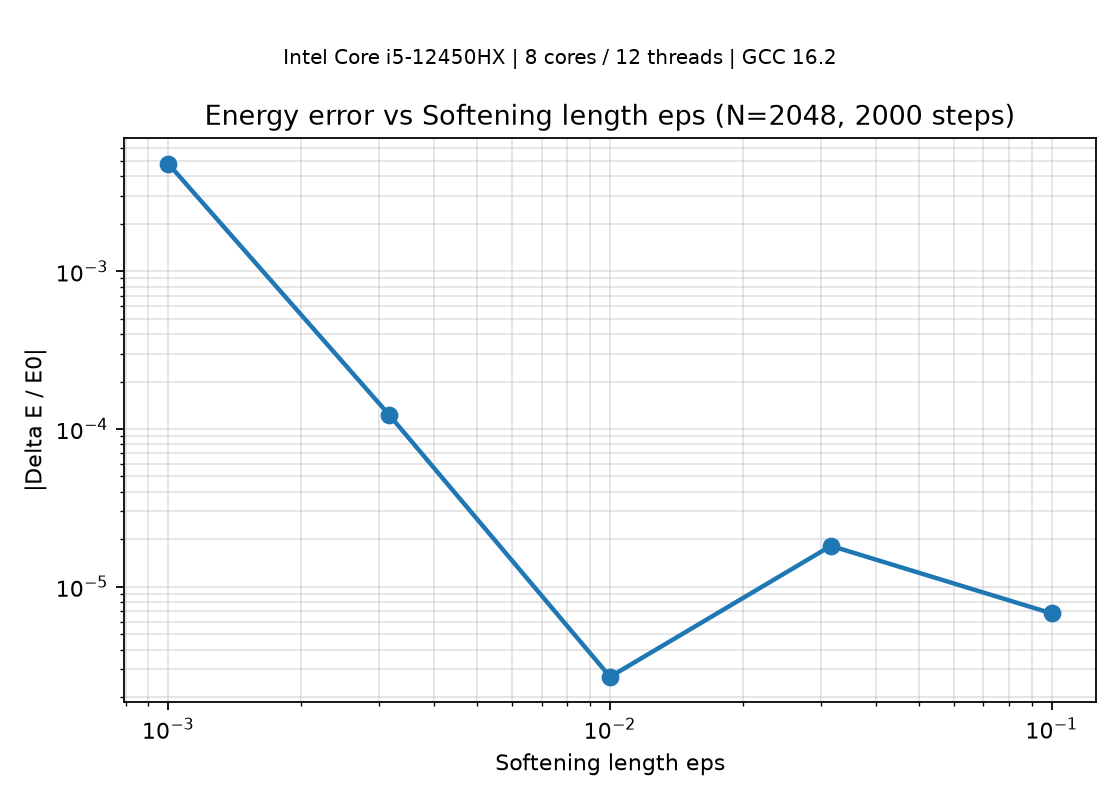
\includegraphics[width=0.85\linewidth]{vvduong_energy_eps}
\caption{Độ lệch năng lượng $|\Delta E/E_0|$ theo $\varepsilon$ ($\Delta t=0.002$).}
\label{fig:vvduong_energy_eps}
\end{figure}

Dữ liệu thô, gồm cả cấu hình máy và tham số từng lần chạy, nằm trong tệp\\ \code{results/vvduong\_energy.csv}.

Khi tăng $\Delta t$ từ 0.002 lên 0.005 và 0.01, độ lệch năng lượng cuối tăng từ $2.685\times10^{-6}$ lên $9.308\times10^{-5}$ và $1.260\times10^{-3}$. Kết quả ở $\Delta t=0.0005$ không nhỏ hơn mọi giá trị khác: $1.700\times10^{-5}$, lớn hơn các giá trị tại 0.001 và 0.002. Điều này cho thấy độ lệch tại một thời điểm cuối không nhất thiết đơn điệu theo bước thời gian; năng lượng của tích phân symplectic có thể dao động và kết quả còn phụ thuộc pha tại thời điểm đo.

Trong phép quét softening, $\varepsilon=0.001$ cho độ lệch lớn nhất $4.799\times10^{-3}$, trong khi $\varepsilon=0.01$ cho $2.685\times10^{-6}$. Các điểm còn lại không tạo thành xu hướng đơn điệu. $\varepsilon$ nhỏ làm lực ở cự ly gần nhạy hơn, còn $\varepsilon$ lớn làm thay đổi đáng kể mô hình thế năng; vì vậy không thể suy ra một quy luật đơn giản chỉ từ một seed và một thời điểm cuối.

\textbf{Giới hạn của phép so sánh:} mỗi lần chạy dùng cùng 2000 bước. Vì vậy, khi thay đổi $\Delta t$, tổng thời gian vật lý $T=2000\Delta t$ cũng thay đổi (từ 1 đến 20 đơn vị thời gian). Các số liệu \texttt{dt} mô tả đúng cấu hình thí nghiệm đã chạy nhưng chưa phải phép so sánh sai số tại cùng một thời điểm vật lý. Một khảo sát hội tụ chặt chẽ hơn cần giữ $T$ cố định và điều chỉnh số bước tỷ lệ nghịch với $\Delta t$. Ngược lại, trong phép quét \texttt{eps}, $\Delta t$ không đổi nên tổng thời gian mô phỏng bằng nhau.

\subsection{Quỹ đạo mô phỏng}

Quỹ đạo được tạo với $N=1024$, 2000 bước, $\Delta t=0.002$, $\varepsilon=0.01$, lưu trạng thái mỗi 20 bước. Hình~\ref{fig:vvduong_energy_orbit} so sánh trạng thái ban đầu và trạng thái ở bước 2000: cụm sao giữ cấu trúc cầu với lõi đặc ở tâm, phù hợp với một cụm Plummer ở trạng thái cân bằng. Ảnh động toàn bộ quỹ đạo (101 khung hình) nằm trong tệp \code{results/vvduong\_energy\_orbit.gif}.

\begin{figure}[H]
\centering
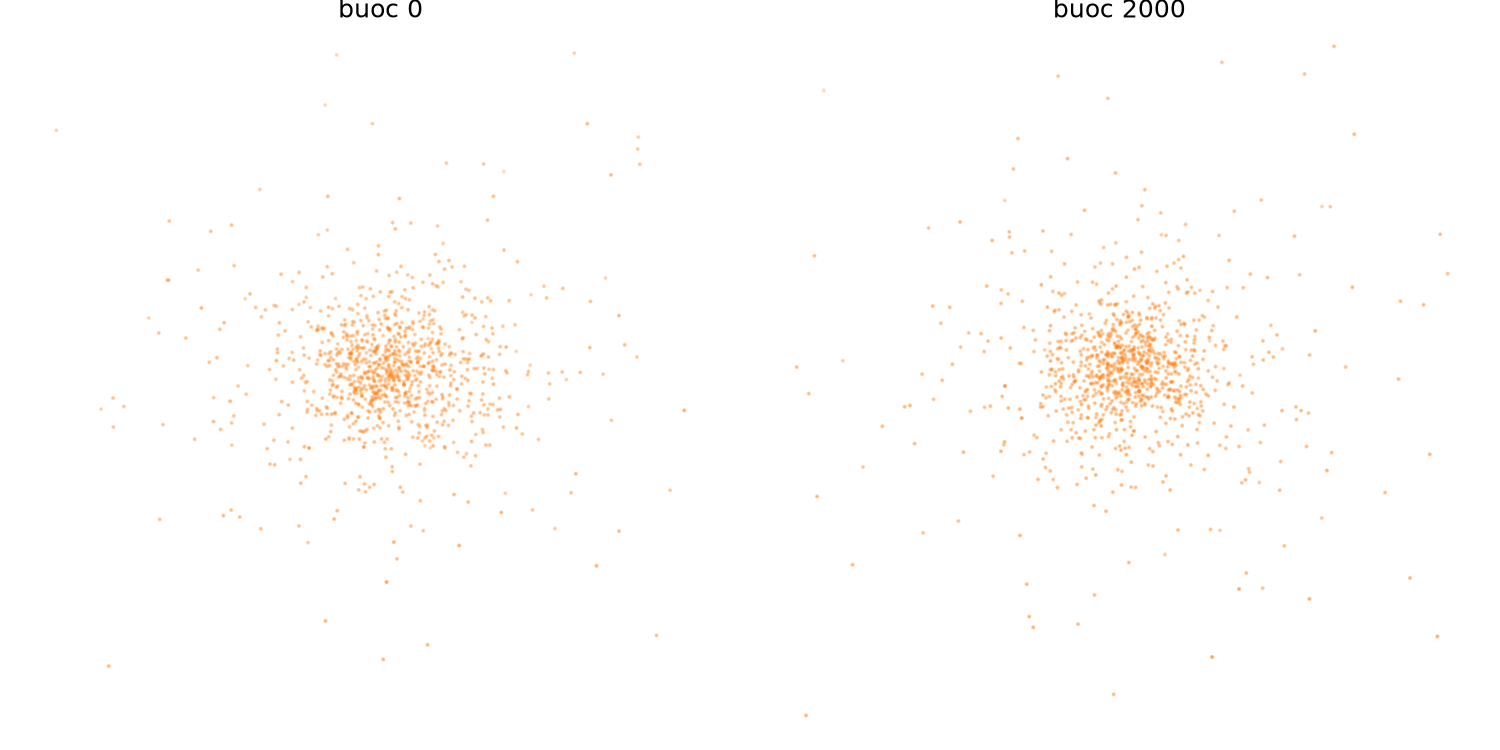
\includegraphics[width=0.85\linewidth]{vvduong_energy_orbit}
\caption{Cụm sao Plummer ở bước 0 và bước 2000 ($N=1024$).}
\label{fig:vvduong_energy_orbit}
\end{figure}

\section{Song song hóa trên CPU bằng OpenMP}
\label{sec:cai-dat-openmp}

\subsection{Cài đặt}

\subsubsection{Chia vòng lặp ngoài}
Theo chiến lược ở Mục~\ref{sec:chien-luoc}, chỉ thị \code{\#pragma omp parallel for}~\cite{openmp52} được đặt trên vòng lặp ngoài $i$ của pha tính gia tốc (Hình~\ref{fig:tuan-tu}); mỗi luồng nhận một đoạn chỉ số $i$ và tính trọn tổng theo $j$ cho các vật thể đó:
\begin{lstlisting}[language=C]
static void nb_acc_omp(const vec4f *pos, vec4f *acc, int n, float eps2)
{
    int i;
#pragma omp parallel for schedule(static) num_threads(nb_num_threads())
    for (i = 0; i < n; i++) nb_body_acc(pos, acc, i, n, eps2);
}
\end{lstlisting}

\subsubsection{Không có xung đột dữ liệu}
Như đã phân tích ở Mục~\ref{sec:phan-tich-nbody}, phân rã theo vật thể đích không gây xung đột dữ liệu. Cụ thể, trong \code{nb\_acc\_omp}:
\begin{itemize}
\item \textbf{Dữ liệu đọc (\texttt{read-only}):} Mảng tọa độ \texttt{pos} chứa vị trí và khối lượng của tất cả các hạt được đọc bởi tất cả các luồng. Không có luồng nào ghi vào \texttt{pos} trong quá trình tính gia tốc.
\item \textbf{Dữ liệu ghi (\texttt{write-private}):} Mỗi vật thể $i$ được gán cố định cho duy nhất một luồng phụ trách. Luồng tính toán gia tốc $\mathbf{a}_i$ và chỉ ghi kết quả vào phần tử \texttt{acc[i]} của riêng nó.
\item \textbf{Kết luận:} Mọi luồng hoạt động trên các địa chỉ bộ nhớ độc lập nhau ở mảng đích. Do đó, \textbf{hoàn toàn không có xung đột dữ liệu}, loại bỏ hoàn toàn nhu cầu sử dụng các cơ chế đồng bộ nặng nề như \texttt{\#pragma omp critical} hay \texttt{\#pragma omp atomic}.
\end{itemize}

\subsubsection{Vector hóa mức lệnh với \texttt{\#pragma omp simd}}
Bên trong hàm tính gia tốc hạt \texttt{nb\_body\_acc}, vòng lặp trong theo $j$ duyệt qua các phần tử liên tục trong bộ nhớ. Ta áp dụng chỉ thị vector hóa SIMD:
\begin{lstlisting}[language=C]
#pragma omp simd reduction(+ : ax, ay, az)
for (j = 0; j < n; j++) {
    const float dx = pos[j].x - xi;
    const float dy = pos[j].y - yi;
    const float dz = pos[j].z - zi;
    const float d2 = dx * dx + dy * dy + dz * dz + eps2;
    const float inv = 1.0f / sqrtf(d2);
    const float s = pos[j].w * inv * inv * inv;
    ax += dx * s;
    ay += dy * s;
    az += dz * s;
}
\end{lstlisting}
Nhờ chỉ thị này, trình biên dịch GCC sinh mã sử dụng các tập thanh ghi vector AVX2 (256-bit, chứa 8 số thực \texttt{float}) và tập lệnh FMA (Fused Multiply-Add). Các biến tích lũy \texttt{ax, ay, az} được thực hiện thông qua toán tử rút gọn \texttt{reduction(+)}, giúp CPU tính toán song song dữ liệu trong cùng một lõi vật lý.

\subsubsection{Khởi động nhóm luồng trước khi đo}
Lần đầu gặp vùng song song, runtime OpenMP phải tạo nhóm luồng và bộ đệm còn trống (cache cold miss). Nếu tính cả chi phí này, kết quả đo bị sai lệch, nhất là khi $N$ nhỏ. Vì vậy chương trình gọi một lần tính gia tốc để khởi động (\emph{warm-up}) trước khi bấm giờ:
\begin{lstlisting}[language=C]
if (parallel) nb_acc_omp(pos, acc, n, eps2);  // warm-up, không tính giờ
\end{lstlisting}

\subsection{Speedup và hiệu suất theo số luồng}

Thí nghiệm đo trên Intel Core i7-13620H (6 lõi P + 4 lõi E, 16 luồng), mỗi cấu hình chạy 3 lần lấy giá trị tốt nhất. Speedup $S_p$ và hiệu suất $E_p$ tính theo \eqref{eq:speedup}, với $T_1$ là thời gian bản tuần tự (Bảng~\ref{tab:omp-threads}, Hình~\ref{fig:ntduong_threads_speedup}).

\begin{table}[!htbp]
\centering\small
\setlength{\tabcolsep}{4pt}
\begin{tabular}{ccccccc}
\toprule
\textbf{$N$} & \textbf{Số luồng ($p$)} & \textbf{Thời gian (s)} & \textbf{ms/bước} & \textbf{GFLOP/s} & \textbf{$S_p$} & \textbf{$E_p$} \\
\midrule
\textbf{2048} & Tuần tự (1T) & 0.011936 & 2.387 & 35.14 & 1.00× & 100.0\% \\
2048 & 1 & 0.012060 & 2.412 & 34.78 & 0.99× & 99.0\% \\
2048 & 2 & 0.006315 & 1.263 & 66.42 & 1.89× & 94.5\% \\
2048 & 4 & 0.003471 & 0.694 & 120.85 & 3.44× & 86.0\% \\
2048 & 8 & 0.003398 & 0.680 & 123.42 & 3.51× & 43.9\% \\
2048 & 16 & 0.003399 & 0.680 & 123.41 & 3.51× & 21.9\% \\
\textbf{4096} & Tuần tự (1T) & 0.046801 & 9.360 & 35.85 & 1.00× & 100.0\% \\
4096 & 1 & 0.047925 & 9.585 & 35.01 & 0.98× & 97.7\% \\
4096 & 2 & 0.024209 & 4.842 & 69.30 & 1.93× & 96.7\% \\
4096 & 4 & 0.012909 & 2.582 & 129.96 & 3.63× & 90.6\% \\
4096 & 8 & 0.014544 & 2.909 & 115.36 & 3.22× & 40.2\% \\
4096 & 16 & 0.012868 & 2.574 & 130.38 & 3.64× & 22.7\% \\
\textbf{8192} & Tuần tự (1T) & 0.197202 & 39.440 & 34.03 & 1.00× & 100.0\% \\
8192 & 1 & 0.193234 & 38.647 & 34.73 & 1.02× & 102.1\% \\
8192 & 2 & 0.096843 & 19.369 & 69.30 & 2.04× & 101.8\% \\
8192 & 4 & 0.050336 & 10.067 & 133.32 & 3.92× & 97.9\% \\
8192 & 8 & 0.044343 & 8.869 & 151.34 & 4.45× & 55.6\% \\
8192 & 16 & \textbf{0.033364} & \textbf{6.673} & \textbf{201.14} & \textbf{5.91×} & \textbf{36.9\%} \\
\textbf{16384} & Tuần tự (1T) & 0.773194 & 154.639 & 34.72 & 1.00× & 100.0\% \\
16384 & 1 & 0.786256 & 157.251 & 34.14 & 0.98× & 98.3\% \\
16384 & 2 & 0.455911 & 91.182 & 58.88 & 1.70× & 84.8\% \\
16384 & 4 & 0.241187 & 48.237 & 111.30 & 3.21× & 80.1\% \\
16384 & 8 & 0.165322 & 33.064 & 162.37 & 4.68× & 58.5\% \\
16384 & 16 & \textbf{0.138587} & \textbf{27.717} & \textbf{193.69} & \textbf{5.58×} & \textbf{34.9\%} \\
\bottomrule
\end{tabular}
\caption{Speedup và hiệu suất OpenMP theo số luồng (i7-13620H, 5 bước).}
\label{tab:omp-threads}
\end{table}

\begin{figure}[H]
\centering
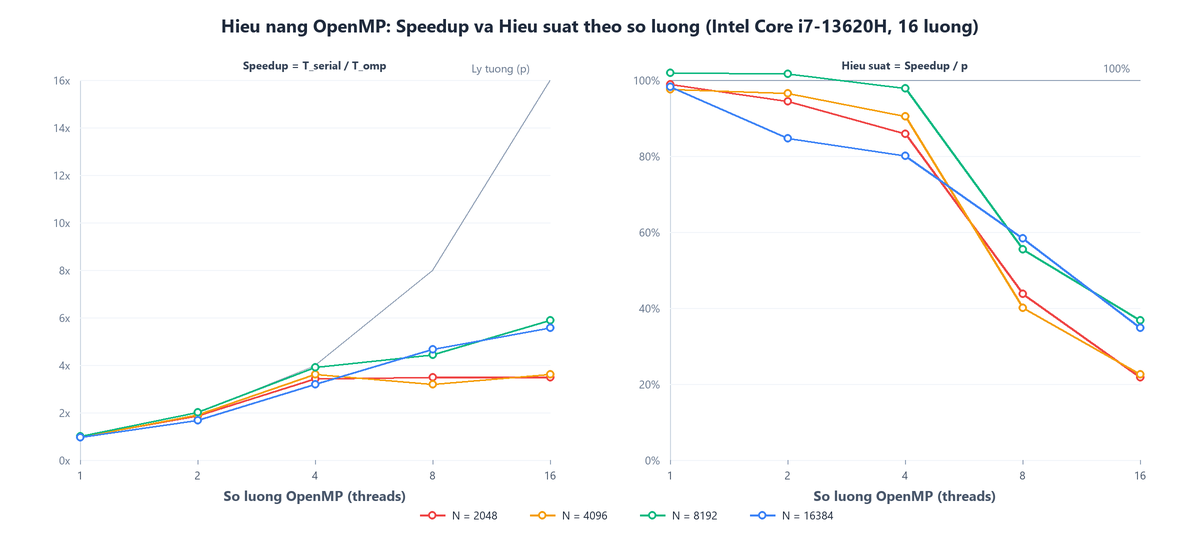
\includegraphics[width=0.85\linewidth]{ntduong_threads_speedup}
\caption{Speedup và hiệu suất OpenMP theo số luồng.}
\label{fig:ntduong_threads_speedup}
\end{figure}

\subsubsection{Vì sao speedup thấp hơn mức lý tưởng 16 lần}

Từ số liệu thực nghiệm, ta thấy Speedup tăng trưởng gần như tuyến tính tuyệt đối từ 1 đến 4 luồng ($S_2 \approx 1.93\times - 2.04\times$, $S_4 \approx 3.44\times - 3.92\times$, hiệu suất $86\% - 100\%$). Tuy nhiên, khi tăng lên 8 và 16 luồng, mức tăng tốc bắt đầu chậm lại và đạt đỉnh ở \textbf{5.91×} ($N=8192$, hiệu năng 201 GFLOP/s).

Hiện tượng này không phải do cài đặt sai mà bắt nguồn từ các đặc tính kiến trúc phần cứng máy tính hiện đại:

\begin{enumerate}
\item \textbf{Kiến trúc nhân bất đối xứng (Heterogeneous Core Topology):}
\begin{itemize}
\item Vi xử lý Intel Core i7-13620H gồm 10 lõi vật lý: 6 lõi P và 4 lõi E.
\item Sáu lõi P hỗ trợ Hyper-Threading (mỗi lõi 2 luồng logic) $\rightarrow$ 12 luồng logic.
\item Bốn lõi E không có Hyper-Threading $\rightarrow$ 4 luồng logic. Tổng cộng là 16 luồng.
\item Khi chạy từ 1 đến 4 luồng, hệ điều hành ưu tiên cấp phát trên 4 lõi P vật lý riêng biệt, nên mỗi luồng độc chiếm toàn bộ tài nguyên tính toán FMA/AVX2 $\rightarrow$ Hiệu suất đạt gần 100\%.
\item Khi chạy 16 luồng, các luồng phải chia sẻ nhân thực (Hyper-Threading trên P-core phải dùng chung các đơn vị thực thi FPU/ALU) và 4 luồng chạy trên E-core có xung nhịp và năng lực tính toán dấu phẩy động thấp hơn đáng kể. Do đó, mức tăng tốc không thể đạt 16×.

\end{itemize}
\item \textbf{Cơ chế giảm xung nhịp Turbo Boost do giới hạn nhiệt và điện năng (Power Throttling):}
\begin{itemize}
\item Khi chạy 1 luồng đơn tuần tự, CPU có thể đẩy xung nhịp của 1 nhân P lên mức tối đa \textbf{4.90 GHz}.
\item Khi chạy đồng thời 16 luồng ở cường độ tính toán AVX2 cao, để giữ công suất tiêu thụ dưới giới hạn gói TDP (45W - 115W), vi xử lý tự động hạ xung nhịp toàn nhân xuống còn khoảng \textbf{2.80 GHz - 3.20 GHz}.
\item Do xung nhịp cơ sở của mỗi nhân khi chạy đa luồng giảm đi khoảng $35\% - 40\%$ so với khi chạy đơn luồng, Speedup đo được tính trên thời gian tuần tự của nhân boost 4.9 GHz sẽ luôn thấp hơn tỷ lệ số luồng thuần túy.

\end{itemize}
\item \textbf{Nghẽn băng thông bộ nhớ (Memory Bandwidth Bottleneck) ở $N$ lớn:}
\begin{itemize}
\item Với $N=16384$, mảng vị trí \texttt{pos} có kích thước $256\text{ KB}$. Mặc dù nằm trong L2/L3 cache, nhưng 16 luồng liên tục đọc đồng thời từ hàng triệu vòng lặp gây áp lực lớn lên các cổng nạp của bộ nhớ đệm (L1/L2 read ports) và bus kết nối liên lõi (Ring Bus).

\end{itemize}
\item \textbf{Kích thước bài toán quá nhỏ khi $N=2048$ và $4096$:}
\begin{itemize}
\item Với $N=2048$, thời gian chạy ở 4 luồng chỉ mất \textbf{0.0035 giây (3.5 ms)}. Ở khoảng thời gian cực ngắn này, chi phí khởi tạo, chuyển ngữ cảnh và đồng bộ luồng tại barrier bắt đầu lấn át thời gian tính toán thực, khiến việc tăng lên 8 hay 16 luồng không làm giảm thêm thời gian thực thi.
\end{itemize}
\end{enumerate}

Đối chiếu với định luật Amdahl \eqref{eq:amdahl}: phần tuần tự của chương trình rất nhỏ khi $N$ lớn, nên giới hạn speedup ở đây không đến từ phần tuần tự mà từ phần cứng: các luồng không có năng lực tính như nhau và cùng tranh chấp tài nguyên chung. Đây là những yếu tố mà mô hình Amdahl lý tưởng không xét đến.

\subsection{Lập lịch và vector hóa SIMD}

Thí nghiệm này so sánh ba chế độ \code{schedule} (Mục~\ref{sec:openmp}) khi bật và tắt vector hóa SIMD, cùng máy i7-13620H, MinGW-W64 GCC 16.2.0 với cờ \code{-O3 -march=native -ffast-math -fopenmp}, 16 luồng, mỗi cấu hình chạy 3 lần lấy kết quả tốt nhất (Bảng~\ref{tab:schedule-simd}).

\begin{table}[H]
\centering\small
\begin{tabular}{cccccc}
\toprule
\textbf{$N$} & \textbf{Schedule} & \textbf{SIMD} & \textbf{ms/bước} & \textbf{GFLOP/s} & \textbf{Tăng tốc SIMD} \\
\midrule
\textbf{2048} & \texttt{static} & \textbf{ON} & \textbf{0.546} & \textbf{153.54} & \textbf{2.50×} \\
2048 & \texttt{static} & OFF & 1.365 & 61.45 & 1.00× \\
2048 & \texttt{dynamic,64} & \textbf{ON} & \textbf{0.581} & \textbf{144.36} & \textbf{1.93×} \\
2048 & \texttt{dynamic,64} & OFF & 1.123 & 74.71 & 1.00× \\
2048 & \texttt{guided,64} & \textbf{ON} & \textbf{0.567} & \textbf{147.92} & \textbf{2.06×} \\
2048 & \texttt{guided,64} & OFF & 1.169 & 71.79 & 1.00× \\
\textbf{4096} & \texttt{static} & \textbf{ON} & \textbf{2.103} & \textbf{159.54} & \textbf{1.88×} \\
4096 & \texttt{static} & OFF & 3.947 & 85.02 & 1.00× \\
4096 & \texttt{dynamic,64} & \textbf{ON} & \textbf{1.586} & \textbf{211.55} & \textbf{2.39×} \\
4096 & \texttt{dynamic,64} & OFF & 3.783 & 88.71 & 1.00× \\
4096 & \texttt{guided,64} & \textbf{ON} & \textbf{1.797} & \textbf{186.73} & \textbf{2.03×} \\
4096 & \texttt{guided,64} & OFF & 3.648 & 91.98 & 1.00× \\
\textbf{8192} & \texttt{static} & \textbf{ON} & \textbf{7.119} & \textbf{188.54} & \textbf{2.09×} \\
8192 & \texttt{static} & OFF & 14.867 & 90.28 & 1.00× \\
8192 & \texttt{dynamic,64} & \textbf{ON} & \textbf{5.849} & \textbf{229.46} & \textbf{2.38×} \\
8192 & \texttt{dynamic,64} & OFF & 13.930 & 96.35 & 1.00× \\
8192 & \texttt{guided,64} & \textbf{ON} & \textbf{6.437} & \textbf{208.51} & \textbf{2.21×} \\
8192 & \texttt{guided,64} & OFF & 14.243 & 94.23 & 1.00× \\
\textbf{16384} & \texttt{static} & \textbf{ON} & \textbf{26.136} & \textbf{205.42} & \textbf{2.19×} \\
16384 & \texttt{static} & OFF & 57.268 & 93.75 & 1.00× \\
16384 & \texttt{dynamic,64} & \textbf{ON} & \textbf{23.148} & \textbf{231.93} & \textbf{2.37×} \\
16384 & \texttt{dynamic,64} & OFF & 54.891 & 97.81 & 1.00× \\
16384 & \texttt{guided,64} & \textbf{ON} & \textbf{25.437} & \textbf{211.06} & \textbf{2.26×} \\
16384 & \texttt{guided,64} & OFF & 57.507 & 93.36 & 1.00× \\
\bottomrule
\end{tabular}
\caption{Thời gian và hiệu năng theo chế độ lập lịch, bật/tắt SIMD (i7-13620H, 16 luồng).}
\label{tab:schedule-simd}
\end{table}

\begin{figure}[H]
\centering
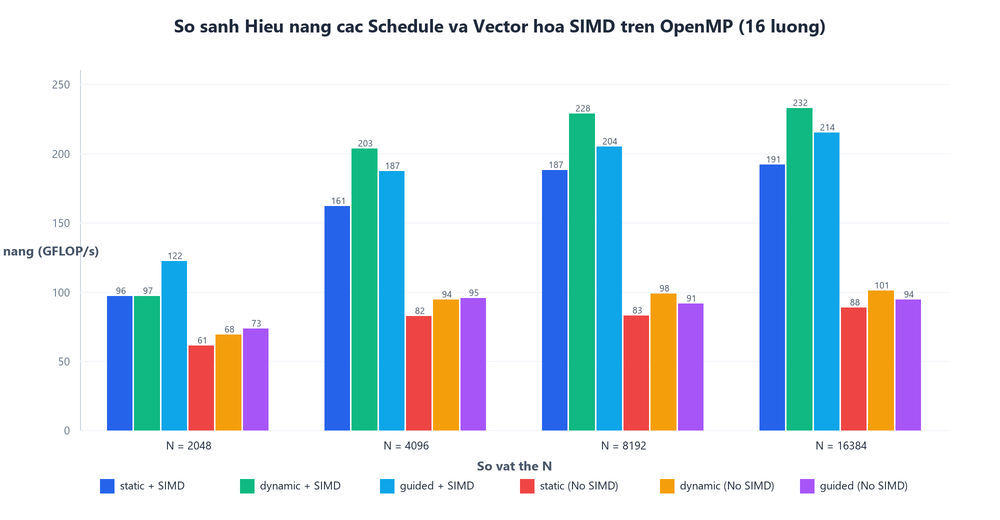
\includegraphics[width=0.85\linewidth]{ntduong_schedule_simd}
\caption{So sánh các chế độ schedule, có và không có SIMD (16 luồng).}
\label{fig:ntduong_schedule_simd}
\end{figure}

\subsubsection{Phân tích}

\begin{enumerate}
\item \textbf{Hiệu ứng vượt trội của SIMD:}
\begin{itemize}
\item Trên tất cả các giá trị $N$, việc bật SIMD (\texttt{\#pragma omp simd reduction}) đem lại mức tăng tốc \textbf{1.88× đến 2.50×} (đạt \textbf{2.09× đến 2.38×} ở $N = 8192\text{--}16384$) so với bản vô hướng không có SIMD.
\item Lưu ý: với \code{-O3 -ffast-math}, GCC tự vector hóa, nên bản OFF (hàm \code{nb\_body\_acc\_nosimd}) được đánh dấu \code{\_\_attribute\_\_((optimize("no-tree-vectorize")))} để đo đúng bản vô hướng. Kiểm tra bằng \code{-fopt-info-vec} cho thấy hàm này không còn vòng lặp nào được vector hóa. Tốc độ bản vô hướng thật (khoảng 90--98 GFLOP/s ở $N = 8192\text{--}16384$) xấp xỉ bản trước khi thêm thuộc tính này, vì ở bản cũ trình biên dịch tự vector hóa với hệ số mở vòng 32, gây tràn thanh ghi YMM ra bộ nhớ ngăn xếp và làm hiệu năng giảm xuống ngang mức vô hướng.
\item Lý do: vòng lặp $j$ của bản SIMD ON được dịch thành lệnh AVX2 256 bit (\code{vrsqrtps}), xử lý 8 tương tác trong một lệnh thay vì từng số vô hướng (\code{vsqrtss}, \code{vmulss}, \code{vdivss}).

\end{itemize}
\item \textbf{Hiện tượng bất đối xứng trên kiến trúc CPU lai (Hybrid P/E Cores):}
\begin{itemize}
\item Theo lý thuyết tính toán song song truyền thống, bài toán All-Pairs có khối lượng mỗi vòng lặp ngoài $i$ là hoàn toàn đồng đều ($N$ tương tác), nên \texttt{schedule(static)} được xem là tối ưu vì chi phí lập lịch bằng 0.
\item Tuy nhiên, số liệu thực nghiệm trên vi xử lý Intel Core i7-13620H lại chỉ ra: \textbf{\texttt{schedule(dynamic, 64)} nhanh hơn \texttt{schedule(static)} rõ rệt} (với $N=16384$, \texttt{dynamic} đạt \textbf{231.93 GFLOP/s}, trong khi \texttt{static} đạt \textbf{205.42 GFLOP/s} — chênh lệch \textasciitilde{}13\%; và với $N=4096\text{--}8192$ đạt \textbf{211.55–229.46 GFLOP/s}, nhanh hơn \texttt{static} tới 21\%–33\%).
\item \textbf{Giải thích cơ chế vật lý:} CPU Intel thế hệ 13 sở hữu 2 loại lõi khác nhau:
\begin{itemize}
\item 6 lõi P (Performance Core): Kiến trúc Raptor Cove, IPC cao, xung nhịp Turbo lên tới 4.9 GHz.
\item 4 lõi E (Efficient Core): Kiến trúc Gracemont, IPC thấp hơn, xung nhịp tối đa chỉ 3.6 GHz.
\item Với \texttt{schedule(static)}, công việc được chia đều thành các đoạn $N/16$. Các luồng chạy trên nhân P-core tính xong sớm hơn nhiều nhưng buộc phải \textbf{chờ đợi (idle wait)} tại rào đồng bộ ngầm của OpenMP để các luồng chạy trên nhân E-core chậm hơn hoàn thành.
\item Với \texttt{schedule(dynamic, 64)}, các nhân P-core sau khi hoàn thành phần của mình sẽ tiếp tục tranh thủ nhận các gói 64 hạt tiếp theo từ hàng đợi chung, giúp toàn bộ hệ thống đạt độ cân bằng tải tối ưu nhất.
\end{itemize}
\end{itemize}
\end{enumerate}

\subsection{Biến thể dùng định luật 3 Newton}

\subsubsection{Ý tưởng và vấn đề xung đột dữ liệu}
Định luật 3 Newton phát biểu rằng lực tác dụng giữa hai vật là trực đối: $\mathbf{F}_{ji} = -\mathbf{F}_{ij}$. Do đó, ta chỉ cần duyệt qua các cặp $(i, j)$ với $i < j$, giảm số phép tính từ $N^2$ xuống còn:
\[ \frac{N(N-1)}{2} \approx \frac{N^2}{2} \text{ cặp tương tác} \]

Tuy nhiên, khi luồng tính toán tương tác giữa cặp $(i, j)$, nó phải cập nhật đồng thời gia tốc cho cả hai vật thể:
\[ \Delta \mathbf{a}_i = + m_j \frac{\mathbf{r}_{ij}}{\left(|\mathbf{r}_{ij}|^2 + \varepsilon^2\right)^{3/2}}, \quad \Delta \mathbf{a}_j = - m_i \frac{\mathbf{r}_{ij}}{\left(|\mathbf{r}_{ij}|^2 + \varepsilon^2\right)^{3/2}} \]

Nếu hai luồng khác nhau cùng tương tác với cùng một vật thể $j$ tại một thời điểm, \textbf{Race Condition sẽ xảy ra} và làm sai lệch nghiêm trọng kết quả.

\subsubsection{Giải pháp: mảng đệm riêng cho từng luồng}
Để song song hóa mà không dùng khóa tuần tự hóa (\texttt{atomic}/\texttt{critical}), ta cấp phát cho mỗi luồng $t \in [0, p-1]$ một mảng đệm gia tốc riêng biệt:
\begin{lstlisting}[language=C]
// mỗi luồng có một mảng đệm \code{my\_acc} gồm N phần tử
vec4f *my_acc = acc_threads + (size_t)tid * (size_t)n;
\end{lstlisting}
Trong vòng lặp song song:
\begin{itemize}
\item Luồng $tid$ chỉ cộng dồn vào \texttt{my\_acc[i]} và \texttt{my\_acc[j]} của riêng nó.
\item Sau khi kết thúc duyệt tất cả các cặp, ta thực hiện bước \textbf{Reduction} (cộng dồn $p$ mảng cục bộ vào mảng \texttt{acc} chung) theo cách song song hóa:
\end{itemize}
\begin{lstlisting}[language=C]
#pragma omp for schedule(static)
for (i = 0; i < n; i++) {
    float sx = 0.0f, sy = 0.0f, sz = 0.0f;
    for (int t = 0; t < p; t++) {
        sx += acc_threads[(size_t)t * n + i].x;
        sy += acc_threads[(size_t)t * n + i].y;
        sz += acc_threads[(size_t)t * n + i].z;
    }
    acc[i].x = sx; acc[i].y = sy; acc[i].z = sz;
}
\end{lstlisting}

\subsubsection{Kết quả đo: all-pairs và Newton 3}

\begin{table}[H]
\centering\small
\begin{tabular}{ccccc}
\toprule
\textbf{$N$} & \textbf{Số luồng} & \textbf{All-pairs (ms/bước)} & \textbf{Newton 3 (ms/bước)} & \textbf{All-pairs nhanh hơn} \\
\midrule
2048 & 1 & 2.427 & 3.352 & 1.38× \\
2048 & 4 & 0.726 & 1.631 & 2.25× \\
2048 & 16 & 0.885 & 1.086 & 1.23× \\
4096 & 1 & 9.506 & 13.899 & 1.46× \\
4096 & 4 & 2.900 & 6.214 & 2.14× \\
4096 & 16 & 2.076 & 2.826 & 1.36× \\
8192 & 1 & 38.813 & 54.367 & 1.40× \\
8192 & 4 & 11.829 & 24.445 & 2.07× \\
8192 & 16 & 7.745 & 11.227 & 1.45× \\
16384 & 1 & 158.180 & 221.712 & 1.40× \\
16384 & 4 & 43.871 & 98.553 & 2.25× \\
16384 & 8 & 31.526 & 60.997 & 1.93× \\
16384 & 16 & \textbf{25.537} & \textbf{41.603} & \textbf{1.63×} \\
\bottomrule
\end{tabular}
\caption{So sánh thời gian all-pairs và biến thể định luật 3 Newton (i7-13620H).}
\label{tab:newton3}
\end{table}

\begin{figure}[H]
\centering
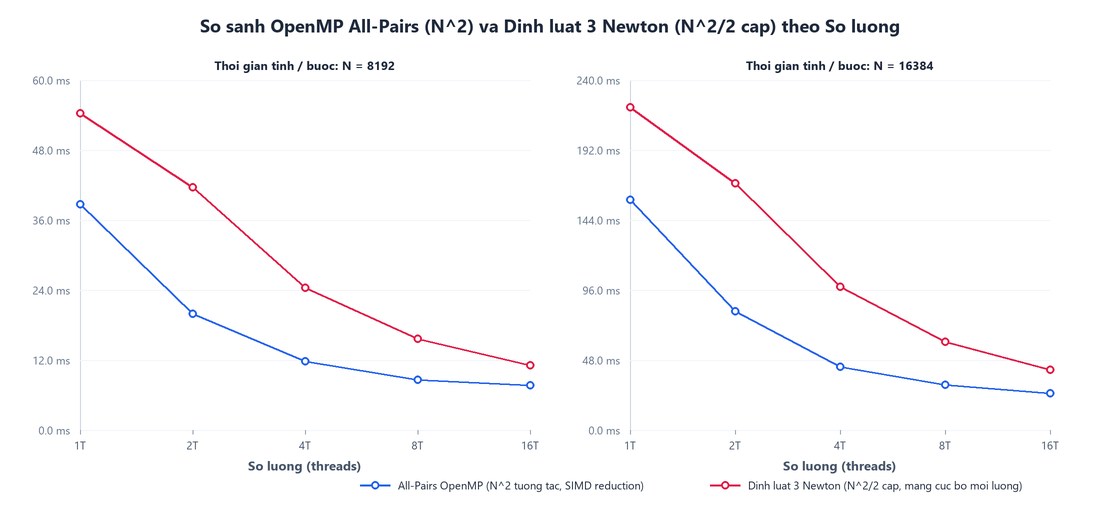
\includegraphics[width=0.85\linewidth]{ntduong_newton3_comparison}
\caption{So sánh All-Pairs và biến thể định luật 3 Newton.}
\label{fig:ntduong_newton3_comparison}
\end{figure}

\subsubsection{Vì sao biến thể Newton 3 chậm hơn}

Mặc dù định luật 3 Newton giảm $50\%$ số phép toán, phiên bản này chạy \textbf{chậm hơn từ 1.2× đến 2.3×} so với all-pairs (Bảng~\ref{tab:newton3}). Kết quả này minh họa sự đánh đổi đã nêu ở Mục~\ref{sec:phan-tich-nbody}: giảm số phép tính nhưng phải trả giá bằng đồng bộ và truy cập bộ nhớ. Có bốn nguyên nhân chính:

\begin{enumerate}
\item \textbf{Mất khả năng vector hóa SIMD liên tục:}
\begin{itemize}
\item Trong All-Pairs, vòng lặp $j$ đọc tuần tự các phần tử liên tiếp từ \texttt{pos[j]} và tích lũy vào một biến thanh ghi cục bộ \texttt{ax, ay, az}. Trình biên dịch dễ dàng vector hóa bằng AVX2 FMA.
\item Trong Newton 3, vòng lặp phải ghi phân tán vào \texttt{my\_acc[j]} ở từng bước lặp. Do $j$ thay đổi, CPU phải thực hiện các thao tác ghi rải rác (\textbf{scatter writes}), triệt tiêu hoàn toàn khả năng vector hóa SIMD đơn giản.
\end{itemize}
\item \textbf{Áp lực bộ nhớ và suy hao Cache (Cache Thrashing):}
\begin{itemize}
\item Bản All-Pairs chỉ có mảng \texttt{pos} (chỉ đọc, nạp vào L2/L3 cache một lần và chia sẻ giữa mọi luồng) và \texttt{acc} ($N \times 16$ byte $\approx 256$ KB với $N=16384$, nằm gọn trong Cache L2).
\item Bản Newton 3 với 16 luồng cần $16 \times N \times 16$ byte $\approx \mathbf{4.19\text{ MB}}$ bộ nhớ ghi riêng. Mười sáu luồng liên tục ghi ngẫu nhiên vào các mảng đệm này, làm tràn bộ đệm L1/L2, đẩy mạnh tỷ lệ cache evictions và làm nghẽn bus bộ nhớ.
\end{itemize}
\item \textbf{Mất cân bằng tải do cấu trúc vòng lặp tam giác:}
\begin{itemize}
\item Do $j$ chạy từ $i+1$ đến $N$, các hạt có $i$ nhỏ cần tính gần $N$ tương tác, trong khi các hạt $i$ gần cuối chỉ cần tính vài tương tác. Dù đã dùng \texttt{schedule(guided)} hay \texttt{dynamic}, việc điều phối khối tam giác vẫn phát sinh overhead lớn hơn nhiều so với lưới chữ nhật đều của All-Pairs.
\end{itemize}
\item \textbf{Chi phí cộng dồn (Reduction Overhead):}
\begin{itemize}
\item Sau khi tính xong, hệ thống phải thực hiện thêm một vòng lặp duyệt $16 \times N$ phần tử để cộng dồn vào \texttt{acc}, tiêu tốn thêm thời gian và băng thông bộ nhớ.
\end{itemize}
\end{enumerate}

\subsection{Nhận xét về phiên bản OpenMP}

\begin{enumerate}
\item \textbf{Hiệu năng đạt được:}
\begin{itemize}
\item Phiên bản OpenMP All-Pairs đạt mức tăng tốc tối đa \textbf{5.91×} tại 16 luồng ($N=8192$), nâng hiệu năng tính toán CPU lên mức \textbf{201.14 GFLOP/s} (so với 34 GFLOP/s của bản tuần tự).
\item Kiểm tra tính đúng đắn (\texttt{-verify}) cho thấy kết quả song song khớp hoàn toàn từng bit với bản tuần tự (sai số tương đối $0.000\text{e}+00$), và năng lượng toàn phần được bảo toàn nghiêm ngặt ($|\Delta E / E_0| \approx 8.78 \times 10^{-7}$).
\end{itemize}
\item \textbf{Vai trò then chốt của SIMD:}
\begin{itemize}
\item Vector hóa SIMD thông qua \texttt{\#pragma omp simd reduction} mang lại mức cải thiện hiệu năng then chốt \textbf{1.9× đến 2.5×} so với bản vô hướng thực thụ (\texttt{no-tree-vectorize}), chứng minh tầm quan trọng của việc kết hợp đa luồng cấp lõi (multithreading) với song song hóa cấp lệnh (SIMD instruction-level parallelism).
\end{itemize}
\item \textbf{Bài học về lập lịch trên CPU lai:}
\begin{itemize}
\item Trên các dòng CPU kiến trúc lai hiện đại (Intel Core gen 12/13/14), \texttt{schedule(dynamic)} giúp cân bằng tải vượt trội giữa nhân P và nhân E, mang lại hiệu năng cao hơn \texttt{schedule(static)} từ \textbf{13\% đến 33\%} (tùy kích thước $N$).
\end{itemize}
\item \textbf{Bài học từ Định luật 3 Newton:}
\begin{itemize}
\item Việc giảm một nửa số phép tính toán học ($N^2/2$) không đồng nghĩa với việc tăng tốc độ thực tế. Chi phí bộ đệm cục bộ (4 MB), xung đột cache, mất vector hóa SIMD và chi phí reduction đã khiến bản Newton 3 chậm hơn bản All-Pairs tiêu chuẩn. Đây là minh chứng rõ ràng cho việc: \textbf{Trong tính toán hiện đại, cấu trúc dữ liệu thân thiện với bộ nhớ đệm (Cache-Friendly) và vector hóa SIMD quan trọng hơn số lượng phép tính thuần túy.}
\end{itemize}
\end{enumerate}

\section{Song song hóa trên GPU bằng CUDA}
\label{sec:cai-dat-cuda}

\subsection{Ánh xạ bài toán lên lưới luồng}

Theo chiến lược ở Mục~\ref{sec:chien-luoc}, \textbf{mỗi luồng CUDA phụ trách một vật thể đích} $i$. Tập $N$ vật thể được chia thành các khối một chiều, mỗi khối $B$ luồng ($B$ = \code{blockDim.x}). Số khối và chỉ số vật thể của mỗi luồng là:
\begin{equation}
\text{gridDim.x} = \left\lceil \frac{N}{B} \right\rceil = \frac{N+B-1}{B}, \qquad
i = \text{blockIdx.x} \times \text{blockDim.x} + \text{threadIdx.x}.
\end{equation}
Do số luồng có thể lớn hơn $N$, mỗi luồng kiểm tra $i<N$ trước khi tính. Mỗi luồng chỉ ghi \code{acc[i]} của mình nên không cần phép toán nguyên tử như \code{atomicAdd}. Chương trình khảo sát $B \in \{64, 128, 256, 512\}$.

Mảng vị trí được lưu dạng \code{float4} như trong GPU Gems 3~\cite{gpugems3}: ba thành phần $x,y,z$ là tọa độ, thành phần $w$ là khối lượng. Một bản ghi 16 byte giúp mỗi luồng đọc cả vị trí và khối lượng trong một lần truy cập. Dữ liệu được sao chép lên GPU một lần trước vòng lặp thời gian và chỉ chép về CPU ở cuối mô phỏng; mỗi bước gồm một kernel tính gia tốc và một kernel cập nhật trạng thái.

\subsection{Kernel naive}

Kernel naive là cách cài đặt trực tiếp: mỗi luồng đọc vị trí vật thể đích vào thanh ghi, rồi duyệt toàn bộ $N$ vật thể nguồn trong global memory để cộng gia tốc. Hàm \code{rsqrtf()} tính nghịch đảo căn bậc hai bằng đơn vị chức năng đặc biệt (SFU) của GPU.

\begin{lstlisting}[language=CUDA]
// Một tương tác (GPU Gems 3, Listing 31-1), khoảng 20 FLOP
__device__ float3 bodyBodyInteraction(float4 bi, float4 bj, float3 ai, float eps2) {
    float3 r = {bj.x - bi.x, bj.y - bi.y, bj.z - bi.z};
    float distSqr = r.x * r.x + r.y * r.y + r.z * r.z + eps2;
    float invDist = rsqrtf(distSqr);
    float s = bj.w * invDist * invDist * invDist;
    ai.x += r.x * s;  ai.y += r.y * s;  ai.z += r.z * s;
    return ai;
}

__global__ void accNaive(const float4 *pos, float4 *acc, int n, float eps2) {
    int i = blockIdx.x * blockDim.x + threadIdx.x;
    if (i >= n) return;
    float4 bi = pos[i];
    float3 a = make_float3(0.0f, 0.0f, 0.0f);
    for (int j = 0; j < n; j++)
        a = bodyBodyInteraction(bi, pos[j], a, eps2);   // pos[j] đọc từ global memory
    acc[i] = make_float4(a.x, a.y, a.z, 0.0f);
}
\end{lstlisting}

\textbf{Hạn chế về bộ nhớ.} Mỗi luồng đọc toàn bộ $N$ bản ghi 16 byte, nên tổng lưu lượng đọc theo mô hình trực tiếp là khoảng $16N^2$ byte, trong khi dữ liệu thực chỉ có $16N$ byte. Như đã phân tích ở Mục~\ref{sec:phan-tich-nbody}, cường độ tính toán khi đó chỉ khoảng $1.25$ FLOP/byte, thấp hơn nhiều so với điểm cân bằng $25.3$ FLOP/byte của T4, nên kernel có nguy cơ bị giới hạn bởi băng thông bộ nhớ. Trên thực tế bộ đệm L1/L2 giữ lại một phần dữ liệu đọc lặp, nhưng kernel naive vẫn phụ thuộc nhiều vào hệ thống bộ nhớ. Cần giảm số lần đọc global memory, và đó là mục tiêu của kernel tiled.

\subsection{Kernel tiled dùng shared memory}

\subsubsection{Ý tưởng}

Kernel tiled áp dụng kỹ thuật chia khối (\emph{tiling}) của GPU Gems 3~\cite{gpugems3}. Tập $N$ vật thể nguồn được chia thành $\lceil N/B \rceil$ \emph{tile}, mỗi tile $B$ vật thể (tile cuối có thể ít hơn). Với mỗi tile, $B$ luồng của một khối phối hợp nạp $B$ vị trí từ global memory vào shared memory, mỗi luồng nạp một phần tử; sau đó mỗi luồng dùng lại cả $B$ phần tử trong shared memory để cộng gia tốc cho vật thể đích của mình (Hình~\ref{fig:tiled}). Các luồng liền kề nạp các địa chỉ liền kề, nên các lần đọc được gộp (coalescing).

\begin{figure}[H]
\centering
\begin{tikzpicture}[>=Stealth, font=\small,
  box/.style={draw, minimum height=0.75cm, align=center},
  lab/.style={font=\footnotesize\itshape, align=center}]
  % global memory
  \node[lab, anchor=east] at (-0.2,3.6) {Global memory\\($N$ vị trí)};
  \foreach \k/\t in {0/Tile 0, 1/Tile 1, 2/Tile 2, 3/$\cdots$, 4/Tile $k$} {
    \node[box, minimum width=2cm, fill=black!5] (g\k) at (\k*2.1+1,3.6) {\t};
  }
  \node[box, minimum width=2cm, fill=orange!25] at (g2) {Tile 2};
  % shared memory
  \node[lab, anchor=east] at (-0.2,1.9) {Shared memory\\(một khối)};
  \node[box, minimum width=4.2cm, fill=orange!25] (sh) at (5.2,1.9) {\code{shPos[0 .. B-1]}};
  \draw[->, thick] (g2.south) -- node[right, lab] {$B$ luồng cùng nạp, mỗi luồng 1 phần tử} (sh.north);
  % threads
  \node[lab, anchor=east] at (-0.2,0.1) {Thanh ghi\\(mỗi luồng)};
  \foreach \k/\t in {0/Luồng 0, 1/Luồng 1, 2/$\cdots$, 3/Luồng $B-1$} {
    \node[box, minimum width=2cm, fill=blue!8] (t\k) at (\k*2.5+1.5,0.1) {\t};
    \draw[->] (sh.south) -- (t\k.north);
  }
  \node[lab] at (5.2,-0.9) {mỗi luồng đọc cả $B$ phần tử của tile, cộng dồn gia tốc cho vật thể $i$ của mình};
\end{tikzpicture}
\caption{Kernel tiled: một tile được nạp một lần cho cả khối rồi dùng lại $B$ lần.}
\label{fig:tiled}
\end{figure}

Theo mô hình lý tưởng, lượng dữ liệu nguồn đọc từ global memory giảm từ khoảng $N^2$ xuống $N^2/B$ phần tử, tức giảm $B$ lần, và cường độ tính toán tăng tương ứng (Mục~\ref{sec:phan-tich-nbody}). Hiệu quả thực tế còn phụ thuộc bộ đệm, chi phí đồng bộ và cách trình biên dịch tối ưu.

\subsubsection{Vòng lặp tile và hai lệnh \texttt{\_\_syncthreads()}}

\begin{lstlisting}[language=CUDA]
extern __shared__ float4 shPos[];          // B phần tử, cấp khi gọi kernel
const float4 bi = (i < n) ? pos[i] : make_float4(0, 0, 0, 0);
for (int tile = 0; tile * blockDim.x < n; tile++) {
    int j = tile * blockDim.x + threadIdx.x;
    shPos[threadIdx.x] = (j < n) ? pos[j] : make_float4(0, 0, 0, 0);
    __syncthreads();                       // (1) chờ cả khối nạp xong
#pragma unroll 8
    for (int k = 0; k < blockDim.x; k++)
        a = bodyBodyInteraction(bi, shPos[k], a, eps2);
    __syncthreads();                       // (2) chờ cả khối dùng xong
}
if (i < n) acc[i] = make_float4(a.x, a.y, a.z, 0.0f);
\end{lstlisting}

Kernel được gọi với kích thước shared memory động \code{B * sizeof(float4)} (tham số thứ ba trong \code{<<<grid, B, B*sizeof(float4)>>>}), nên cùng một mã chạy được với mọi $B$. Khác với kernel naive, luồng có $i \ge N$ \emph{không} được thoát sớm, vì mọi luồng của khối đều phải nạp tile và đi qua \code{\_\_syncthreads()}. Phần tử đệm ngoài phạm vi được gán khối lượng 0 nên đóng góp 0 vào gia tốc, không cần rẽ nhánh trong vòng trong. Hai lệnh đồng bộ có vai trò khác nhau và đều cần thiết~\cite{gpugems3}:
\begin{itemize}
\item \textbf{Lần (1) -- đọc sau ghi (RAW):} bảo đảm mọi luồng trong khối đã ghi xong phần tử của mình vào \code{shPos} trước khi bất kỳ luồng nào đọc \code{shPos[j]}. Thiếu lệnh này, một số warp có thể đọc dữ liệu chưa được nạp hoặc dữ liệu của tile cũ.
\item \textbf{Lần (2) -- ghi sau đọc (WAR):} bảo đảm không còn luồng nào đang đọc tile hiện tại trước khi tile tiếp theo được nạp đè lên cùng vùng nhớ. Thiếu lệnh này, warp chạy nhanh có thể ghi đè dữ liệu mà warp khác vẫn đang dùng.
\end{itemize}

\subsection{Kết quả trên Tesla T4}

Thí nghiệm chạy trên Google Colab: Tesla T4, driver 580.82.07, CUDA 13.0, \code{nvcc -O3}, số thực FP32; CPU của máy ảo là Intel Xeon 2.00 GHz, Linux 6.6. Phép so sánh naive--tiled dùng 5 bước, mỗi cấu hình đo 3 lần lấy lần nhanh nhất, $N$ từ 1024 đến 131072 và $B \in \{64,128,256,512\}$. Phép đo chi phí truyền dữ liệu dùng 10 bước, $B=256$.

\subsubsection{Kernel naive và tiled}

Bảng~\ref{tab:naive-tiled} cho thời gian 5 bước và hiệu năng của hai kernel với $B=256$; Hình~\ref{fig:gpu_speedup} so sánh speedup của OpenMP 16 luồng và hai kernel CUDA so với bản tuần tự (trục tung thang logarit).

\begin{table}[H]
\centering\small
\begin{tabular}{rrrrrr}
\toprule
\textbf{$N$} & \textbf{Naive (ms)} & \textbf{Tiled (ms)} & \textbf{Tiled/naive} & \textbf{GFLOP/s naive} & \textbf{GFLOP/s tiled} \\
\midrule
1024 & 0.315 & 0.205 & 1.54× & 332.54 & 511.52 \\
2048 & 0.625 & 0.391 & 1.60× & 670.93 & 1073.74 \\
4096 & 1.277 & 0.751 & 1.70× & 1313.48 & 2233.39 \\
8192 & 2.489 & 1.491 & 1.67× & 2696.09 & 4501.10 \\
16384 & 7.214 & 5.741 & 1.26× & 3720.98 & \textbf{4675.87} \\
32768 & 28.685 & 24.457 & 1.17× & 3743.21 & 4390.29 \\
65536 & 131.047 & 109.366 & 1.20× & 3277.41 & 3927.16 \\
131072 & 515.285 & 442.754 & 1.16× & 3334.05 & 3880.23 \\
\bottomrule
\end{tabular}
\caption{Thời gian 5 bước và hiệu năng của kernel naive và tiled trên Tesla T4 ($B=256$).}
\label{tab:naive-tiled}
\end{table}

\begin{figure}[H]
\centering
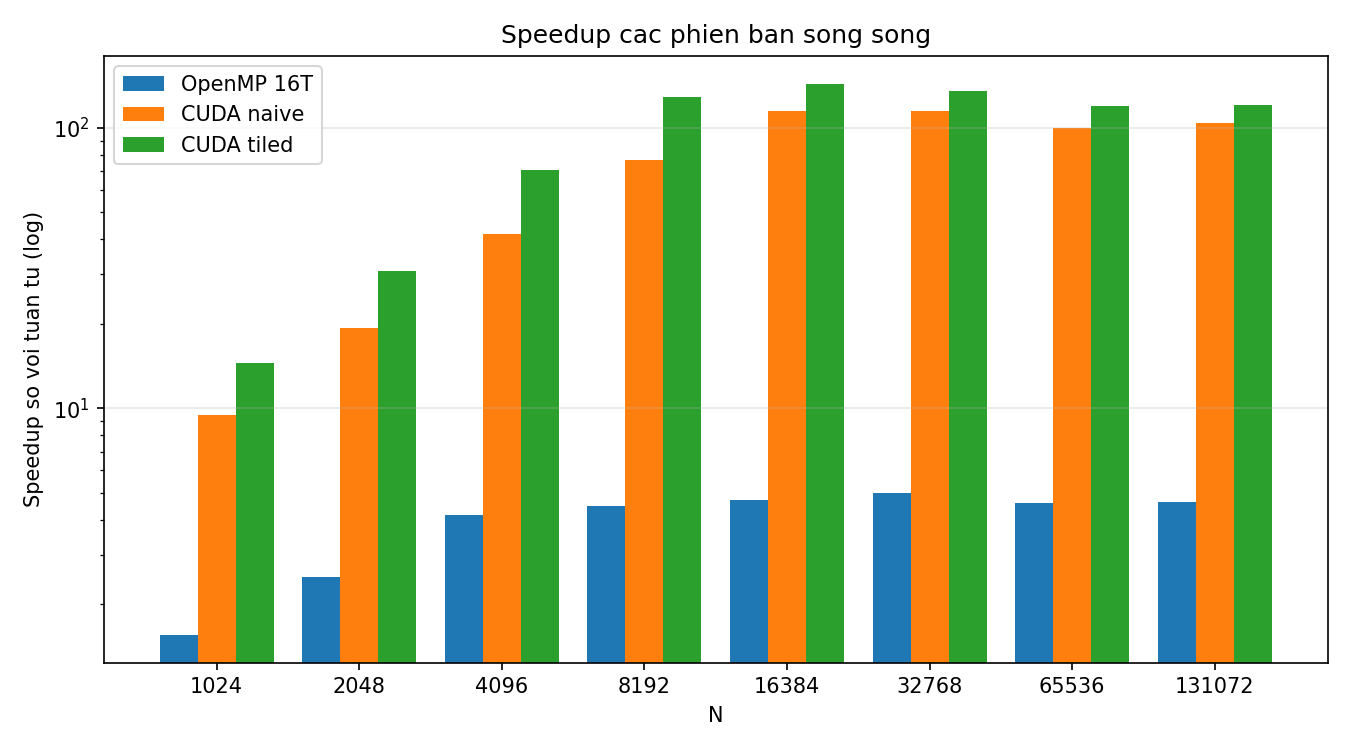
\includegraphics[width=0.85\linewidth]{gpu_speedup}
\caption{Speedup so với bản tuần tự của OpenMP 16 luồng, CUDA naive và CUDA tiled.}
\label{fig:gpu_speedup}
\end{figure}

Kernel tiled nhanh hơn naive ở mọi kích thước, từ 1.16 đến 1.70 lần. Lợi ích rõ nhất khi $N \le 8192$ (1.54--1.70 lần) nhờ tái sử dụng dữ liệu trong shared memory. Khi $N \ge 16384$, khoảng cách thu hẹp còn khoảng 1.2 lần: bộ đệm L1/L2 của Turing giữ lại phần lớn dữ liệu mà kernel naive đọc lặp, nên naive không còn bị giới hạn nặng bởi băng thông như mô hình lý tưởng dự đoán; trong khi đó tiled phải trả thêm chi phí nạp tile và đồng bộ.

\subsubsection{Ảnh hưởng của kích thước khối}

\begin{table}[H]
\centering\small
\begin{tabular}{rrrr}
\toprule
\textbf{$B$} & \textbf{Thời gian (ms/5 bước)} & \textbf{Tương tác ($10^9$/s)} & \textbf{Hiệu năng (GFLOP/s)} \\
\midrule
64 & 450.288 & 190.77 & 3815.31 \\
128 & 449.339 & 191.17 & 3823.36 \\
256 & \textbf{442.754} & \textbf{194.01} & \textbf{3880.23} \\
512 & 460.908 & 186.37 & 3727.40 \\
\bottomrule
\end{tabular}
\caption{Ảnh hưởng của kích thước khối đến kernel tiled ($N=131072$).}
\label{tab:block-size}
\end{table}

\begin{figure}[H]
\centering
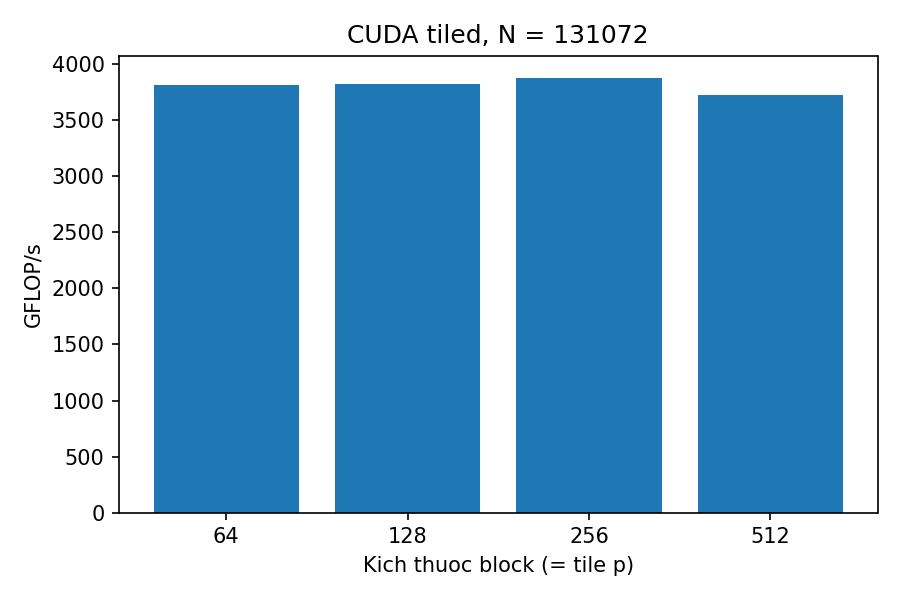
\includegraphics[width=0.8\linewidth]{block_size}
\caption{Hiệu năng kernel tiled theo kích thước khối ($N=131072$).}
\label{fig:block_size}
\end{figure}

$B=256$ cho kết quả tốt nhất, nhưng bốn cấu hình chỉ chênh nhau dưới 4\% (Bảng~\ref{tab:block-size}). Khối nhỏ (64, 128) tái sử dụng mỗi tile ít lần hơn; khối lớn (512) dùng nhiều tài nguyên hơn trên mỗi SM, giảm số khối chạy đồng thời (occupancy). Lựa chọn kích thước khối là cân bằng giữa hai yếu tố này; $B=256$ phù hợp trong phạm vi thí nghiệm, không phải giá trị tối ưu cho mọi GPU.

\subsubsection{Chi phí truyền dữ liệu}

\begin{table}[H]
\centering\small
\begin{tabular}{rrrrrr}
\toprule
\textbf{$N$} & \textbf{H2D (ms)} & \textbf{D2H (ms)} & \textbf{Kernel (ms)} & \textbf{Tỷ lệ truyền} & \textbf{GFLOP/s} \\
\midrule
4096 & 0.090 & 0.066 & 2.569 & 5.72\% & 1306.18 \\
16384 & 0.288 & 0.178 & 15.663 & 2.89\% & 3427.62 \\
65536 & 0.780 & 0.684 & 212.138 & 0.69\% & 4049.23 \\
131072 & 1.230 & 1.231 & 839.962 & 0.29\% & 4090.63 \\
\bottomrule
\end{tabular}
\caption{Chi phí sao chép H2D/D2H so với thời gian tính của kernel tiled (10 bước, $B=256$, một lần đo).}
\label{tab:h2d}
\end{table}

Tỷ lệ thời gian truyền trong tổng thời gian giảm từ 5.72\% ($N=4096$) xuống 0.29\% ($N=131072$), vì lượng dữ liệu truyền tăng theo $O(N)$ còn khối lượng tính tăng theo $O(N^2)$ (Bảng~\ref{tab:h2d}). Kết quả này phù hợp với phân tích theo định luật Gustafson ở Mục~\ref{sec:do-do}: phần không song song hóa được co lại khi bài toán lớn lên. Điều kiện để đạt được tỷ lệ thấp này là dữ liệu được giữ trên GPU suốt mô phỏng; nếu sao chép qua lại ở mỗi bước, chi phí PCIe sẽ đáng kể. Lần đo này là một lần chạy riêng 10 bước, chỉ dùng để đánh giá tỷ lệ sao chép, không thay cho số liệu 5 bước ở Bảng~\ref{tab:naive-tiled}.

\subsection{Nhận xét về phiên bản CUDA}

\begin{itemize}
\item \textbf{Đối chiếu với lý thuyết hiệu năng.} Kernel tiled đạt cao nhất 4675.87 GFLOP/s ($N=16384$), khoảng 57.7\% đỉnh FP32 lý thuyết 8100 GFLOP/s của T4; ở $N \ge 65536$, hiệu năng khoảng 3880--4090 GFLOP/s (48--51\% đỉnh). Theo mô hình roofline \eqref{eq:roofline}, kernel tiled với $B=256$ có cường độ tính toán vượt xa điểm cân bằng, tức là bị giới hạn bởi tính toán chứ không bởi bộ nhớ.
\item \textbf{Khoảng cách tới đỉnh lý thuyết} đến từ: hàm \code{rsqrtf()} chạy trên đơn vị SFU có thông lượng thấp hơn FP32 thường; chi phí hai lệnh \code{\_\_syncthreads()} mỗi tile; chi phí điều khiển vòng lặp; occupancy bị giới hạn bởi thanh ghi và shared memory; vòng trong mới chỉ mở 8 lần (\code{\#pragma unroll 8}) và mỗi luồng mới tính một vật thể, chưa thử cho mỗi luồng tính nhiều vật thể (thread coarsening). Ở $N$ rất lớn, T4 (giới hạn 70 W) có thể hạ xung khi kernel chạy liên tục hàng trăm mili giây.
\item \textbf{So với GPU Gems 3.} Tài liệu gốc báo cáo khoảng 250 GFLOP/s trên GeForce 8800 GTX~\cite{gpugems3}; kết quả trên T4 cao hơn khoảng 18.7 lần, chủ yếu nhờ phần cứng mới hơn với nhiều nhân CUDA hơn.
\end{itemize}

\section{So sánh tổng hợp CPU và GPU}
\label{sec:tong-hop}

\subsection{Kết quả tổng hợp}

Bảng~\ref{tab:tong-hop} tổng hợp thời gian mỗi bước của bốn phiên bản trong cùng một lần đo (môi trường ở Bảng~\ref{tab:moi-truong}); Hình~\ref{fig:time_vs_n} vẽ các số liệu này trên thang log--log.

\begin{table}[H]
\centering\small
\setlength{\tabcolsep}{3pt}
\begin{tabular}{rrrrrrrr}
\toprule
\textbf{$N$} & \textbf{Tuần tự} & \textbf{OpenMP 16} & \textbf{OpenMP/} & \textbf{CUDA naive} & \textbf{CUDA tiled} & \textbf{Tiled/} & \textbf{Tiled/} \\
 & \textbf{(ms)} & \textbf{luồng (ms)} & \textbf{tuần tự} & \textbf{(ms)} & \textbf{(ms)} & \textbf{tuần tự} & \textbf{OpenMP} \\
\midrule
1024 & 0.611 & 0.383 & 1.6× & 0.063 & 0.041 & 14.9× & 9.3× \\
2048 & 2.464 & 1.171 & 2.1× & 0.125 & 0.078 & 31.5× & 15.0× \\
4096 & 10.006 & 2.844 & 3.5× & 0.255 & 0.150 & 66.6× & 18.9× \\
8192 & 39.446 & 9.065 & 4.4× & 0.498 & 0.298 & 132.3× & 30.4× \\
16384 & 158.032 & 40.023 & 3.9× & 1.443 & 1.148 & 137.6× & 34.9× \\
32768 & 693.889 & 146.524 & 4.7× & 5.737 & 4.891 & 141.9× & 30.0× \\
65536 & 2742.200 & 629.848 & 4.4× & 26.209 & 21.873 & 125.4× & 28.8× \\
131072 & 11693.782 & 2431.867 & 4.8× & 103.057 & 88.551 & 132.1× & 27.5× \\
\bottomrule
\end{tabular}
\caption{Thời gian mỗi bước và speedup của bốn phiên bản. CPU: $N \le 16384$ đo 5 bước, $N \ge 32768$ đo 1 bước; GPU: 5 bước, $B=256$; mỗi cấu hình lấy lần nhanh nhất trong 3 lần (nguồn: \code{results/summary.md}).}
\label{tab:tong-hop}
\end{table}

\begin{table}[H]
\centering\small
\begin{tabular}{lrr}
\toprule
\textbf{Phiên bản ($N=16384$)} & \textbf{GFLOP/s} & \textbf{So với tuần tự} \\
\midrule
Tuần tự & 34 & 1× \\
OpenMP 16 luồng & 134 & 3.9× \\
CUDA naive & 3721 & 110× \\
CUDA tiled & 4676 & 138× \\
\bottomrule
\end{tabular}
\caption{Hiệu năng của bốn phiên bản ở $N=16384$ (quy ước 20 FLOP/tương tác).}
\label{tab:gflops}
\end{table}

\begin{figure}[H]
\centering
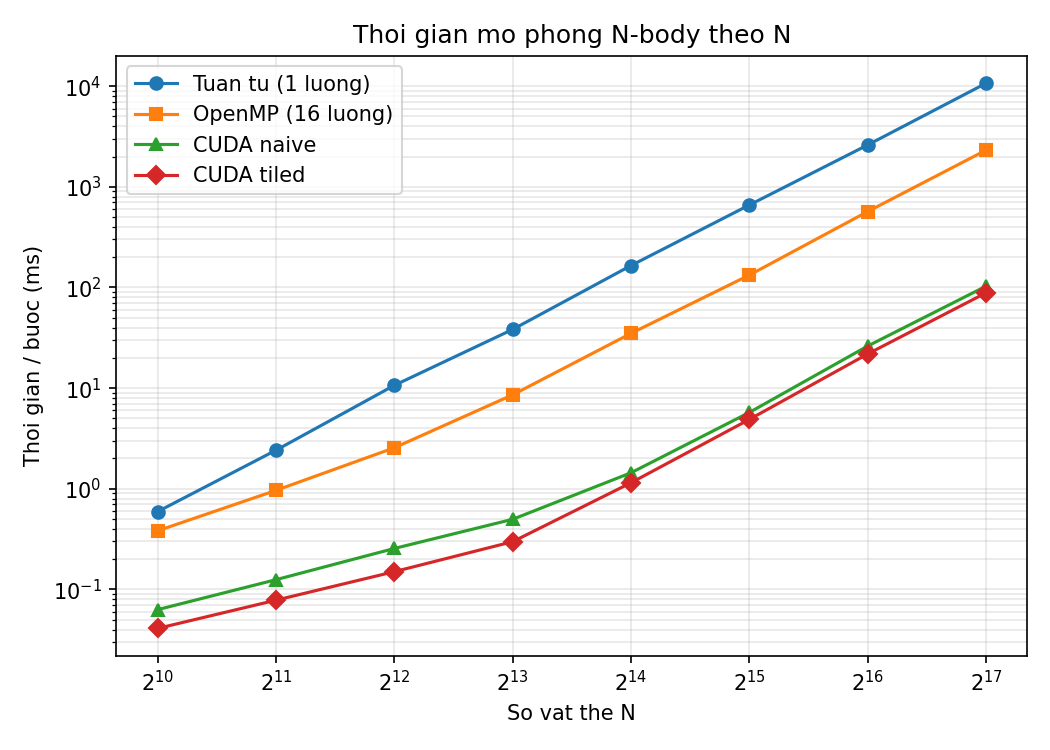
\includegraphics[width=0.85\linewidth]{time_vs_n}
\caption{Thời gian mỗi bước theo $N$ của bốn phiên bản (thang log--log).}
\label{fig:time_vs_n}
\end{figure}

\subsection{Nhận xét}

\textbf{Độ phức tạp $O(N^2)$.} Trên Hình~\ref{fig:time_vs_n}, mỗi lần $N$ tăng gấp đôi thì thời gian tuần tự tăng khoảng 4 lần (ví dụ $39.4 \to 158.0 \to 693.9$ ms), tức độ dốc khoảng 2, đúng với độ phức tạp $O(N^2)$. Các đường OpenMP và CUDA cũng có độ dốc khoảng 2 khi $N$ đủ lớn: song song hóa chỉ dịch đường thẳng xuống dưới, không thay đổi bậc của bài toán.

\textbf{OpenMP.} Với 16 luồng trên i5-12500H, OpenMP nhanh hơn tuần tự 4.4--4.8 lần khi $N \ge 8192$; thí nghiệm riêng trên i7-13620H đạt tối đa 5.91 lần (Mục~\ref{sec:cai-dat-openmp}). Cả hai đều thấp hơn nhiều so với 16 lần lý tưởng vì CPU lai chỉ có 4--6 lõi P, các lõi E chậm hơn và xung nhịp giảm khi nhiều lõi cùng chạy. Với $N$ nhỏ (1024--2048), chi phí tạo và đồng bộ luồng chiếm tỷ lệ lớn nên speedup chỉ 1.6--2.1 lần.

\textbf{GPU so với CPU.} CUDA tiled nhanh hơn bản tuần tự 125--142 lần và nhanh hơn OpenMP 16 luồng 28--35 lần khi $N \ge 8192$. Với $N$ nhỏ, lợi thế giảm còn 15 lần ($N=1024$): lưới chỉ có 4 khối 256 luồng, không đủ lấp đầy 40 SM của T4. Đây là lý do đường CUDA trên Hình~\ref{fig:time_vs_n} thoải hơn (độ dốc nhỏ hơn 2) ở vùng $N \le 8192$. Điều này phù hợp với định luật Gustafson: GPU chỉ phát huy hết khi bài toán đủ lớn.

\textbf{Lưu ý về phép so sánh.} CPU và GPU được đo trên hai máy khác nhau (laptop và Google Colab); CPU dùng \code{-ffast-math}, GPU dùng \code{-use\_fast\_math} (hàm \code{rsqrtf}). Vì vậy các tỷ số CPU--GPU phản ánh bậc độ lớn, không phải phép so sánh trên cùng một hệ thống.
